\documentclass[11pt, addpoints, answers]{exam}
\usepackage{amsmath, amssymb}
% \usepackage{amsmath, amssymb, euler}
\usepackage{xcolor}
\usepackage{tikz}
\usetikzlibrary{positioning, arrows.meta}
\usepackage{complexity} % For HW12 complexity classes
\usepackage{caption}
\usepackage{float}

\usepackage{blindtext} % For hyperlink
\usepackage{hyperref}

% headers, footers, titles
\newcommand{\CourseName}{CS101 Algorithms and Data Structures}
\newcommand{\HomeworkNO}{Homework 12}
\newcommand{\DueDate}{Due date: 23:59, January 1st, 2025}

\pagestyle{headandfoot}
\runningheadrule{}
\runningheader{\CourseName}{\HomeworkNO}{\DueDate}
\runningfooter{}{\thepage}{}

\title{
	\CourseName\\
	Fall 2024\\
	\HomeworkNO
}
\author{}
\date{\DueDate}

% formats of questions, choices, points, etc.
\qformat{\bf\thequestion. (\totalpoints\ points) \thequestiontitle\hfill}
\pointname{'}
\CorrectChoiceEmphasis{\bf\color{blue}}
\SolutionEmphasis{\color{blue}}

% We frequently use this font.
\newcommand{\ttt}{\texttt}
\newcommand{\bluett}[1]{\textcolor{blue}{\ttt{#1}}}
\newcommand{\red}[1]{\textcolor{red}{#1}}
\newcommand{\complete}[1]{\textsf{#1}\text{-}\textsf{Complete}}
\newcommand{\hard}[1]{\textsf{#1}\text{-}\textsf{Hard}}
\newcommand{\pnp}{\textsf{P}=\textsf{NP}}
\newcommand{\sat}[1]{\textsf{#1}\text{-}\SAT}
\newcommand{\aseq}[1]{\langle{#1}\rangle}
\begin{document}

\maketitle

\begin{enumerate}
	\item Please write your solutions in English.
	\item Submit your solutions to gradescope.com.
	\item Set your FULL name to your Chinese name and your STUDENT ID correctly in Account Settings.
	\item If you want to submit a handwritten version, scan it clearly. \ttt{CamScanner} is recommended.
	\item When submitting, match your solutions to the problems correctly.
	\item No late submission will be accepted.
	\item Violations to any of the above may result in zero points.
 	\item You are recommended to finish this homework with \LaTeX.
\end{enumerate}

\newpage

\begin{questions}
    \titledquestion{Tutorial on how to prove that a particular problem is in $\complete{\NP}$}[0]

To prove problem $A$ is in $\complete{\NP}$, your answer should include:
\begin{enumerate}

  \item Prove that problem $A$ is in $\NP$ by showing: What your {\color{red} polynomial-size} certificate is and what your {\color{red} polynomial-time} certifier is.

  \item Choose a problem $B$ in $\complete{\NP}$ to reduce from.
  
  \item Construct your {\color{red} polynomial-time many-one reduction} $f$ that maps instances of problem $B$ to instances of problem $A$. 
  
  (polynomial-time many-one reduction = polynomial transformation = Karp reduction, see presenter notes of page 7 \& 61 in lecture slides (.pptx file) for more details.) 

  \item Prove the correctness of your reduction (i.e. Prove that your reduction $f$ do map $yes$-instance of problem $B$ to $yes$-instance of problem $A$ and map $no$-instance of problem $B$ to $no$-instance of problem $A$) by showing:
  \begin{enumerate}
      \item $x$ is a $yes$-instance of problem $B$ $\Rightarrow$ $f(x)$ is a $yes$-instance of problem $A$.
      \item $x$ is a $yes$-instance of problem $B$ $\Leftarrow$ $f(x)$ is a $yes$-instance of problem $A$.
  \end{enumerate}
\end{enumerate}
{\textbf{Proof Example}: Prove that the decision version of $\mathsf{Set\text{-}Cover}$ is in $\complete{\NP}$.}

 Recall that the $yes$-instances of the decision version of $\mathsf{Set\text{-}Cover}$ is:
\begin{align*}
\mathsf{Set\text{-}Cover}= \left\{\langle{U, S_1, \ldots, S_n, k \rangle}~\middle|~~~
 \begin{aligned}
     &n \in \mathbb{Z}^+, S_1, \ldots, S_n \subseteq U \text{ and there exist $k$ sets } S_{i_1}, \ldots, \\& S_{i_k} 
     \text{that cover all of $U$, i.e., }
     S_{i_1} \cup S_{i_2} \cup \dots \cup S_{i_k} = U
 \end{aligned}
\right\}
\end{align*}

To prove that the decision version of $\mathsf{Set\text{-}Cover}$ is in $\complete{\NP}$, we follow these steps:
 
\begin{enumerate}
    \item \textbf{Membership in $\NP$}:
        \begin{enumerate}
        \item A set of indices $\left\{i_1, \dots, i_k\right\} \subseteq \left\{1, 2, \dots, n\right\}$, whose size is polynomial of input size .
        \item Check whether $S_{i_1} \cup S_{i_2} \cup \dots \cup S_{i_k} = U$, whose run-time is polynomial of input size.
        \end{enumerate}
    \item \textbf{Reduction from $\mathsf{Vertex\text{-}Cover}$}:
        \begin{enumerate}
            \item We choose the decision version of $\mathsf{Vertex\text{-}Cover}$ as the problem to reduce from.
            \begin{equation*}
            \mathsf{Vertex\text{-}Cover} = \left\{\langle{G,k'\rangle}~\middle|~~~
            \begin{aligned}
                &\text{$G$ is an undirected graph and there exists a set of} \\&\text{$k'$ vertices that touches all edges in $G$.}
            \end{aligned}\right\}
            \end{equation*}
            \item Given an undirected graph $G = (V, E)$ and a positive integer $k' \in \mathbb{Z}^+$, we construct the reduction $f(\langle G, k' \rangle) = \langle U, S_1, \ldots, S_n, k \rangle$ as follows: $U = E$. $n = |V|$ and $k = k'$. For each $i \in \{1, \ldots, n\}$, $S_i = \{e \in E \mid e = (v_i, u) \text{ for some } u \in V \setminus \{v_i\}\}$.
            \item We prove the correctness of the reduction:
                \begin{enumerate}
                    \item[``$\Rightarrow$'':] If $\langle G, k' \rangle$ is a $yes$-instance of $\mathsf{Vertex\text{-}Cover}$, then there exists a set $V^* = \{v_{i_1}, \ldots, v_{i_{k'}}\}$ of vertices that covers all edges. By construction, $\{S_{i_1}, \ldots, S_{i_{k'}}\}$ covers all edges in $U$, so $\langle U, S_1, \ldots, S_n, k \rangle$ is a $yes$-instance of $\mathsf{Set\text{-}Cover}$.
                    \item[``$\Leftarrow$'':] Conversely, if $\langle U, S_1, \ldots, S_n, k \rangle$ is a $yes$-instance of $\mathsf{Set\text{-}Cover}$, then there exists a set $\{S_{i_1}, \ldots, S_{i_k}\}$ of sets that covers all edges in $U$. By construction, the corresponding set of vertices $\{v_{i_1}, \ldots, v_{i_k}\}$ covers all edges in $G$, so $\langle G, k' \rangle$ is a $yes$-instance of $\mathsf{Vertex\text{-}Cover}$.
                \end{enumerate}
        \end{enumerate}
\end{enumerate}
 
Hence, the decision version of $\mathsf{Set\text{-}Cover}$ is in $\complete{\NP}$.

\newpage
In fact, any two problems in $\P$ can reduce to each other in polynomial time, indicating they share the same ``hardness.'' To illustrate, consider decision problems $A$ and $B$ in $\mathcal{P}$. Given an instance $x$ of $A$:
 
\begin{enumerate}
    \item Prepare polynomial-time copies of known $yes$- and $no$-instances of $B$.
    \item Determine if $x$ is a $yes$-instance of $A$ in polynomial time.
    \item Return the corresponding $yes$- or $no$-instance of $B$.
\end{enumerate}
 
For example, let $A$ be the minimum spanning tree cost problem and $B$ be the shortest path cost problem in undirected weighted graphs. Given an instance $G$ of $A$:
 
\begin{enumerate}
    \item Prepare graphs $G_1$ and $G_2$ with known shortest path costs relative to $c'$.
    \item Find $G$'s minimum spanning tree cost using Kruskal's algorithm and compare it with $c$.
    \item Return $G_1$ if the cost is no more than $c$, otherwise return $G_2$.
\end{enumerate}

A brief map of common NP-Complete problems:

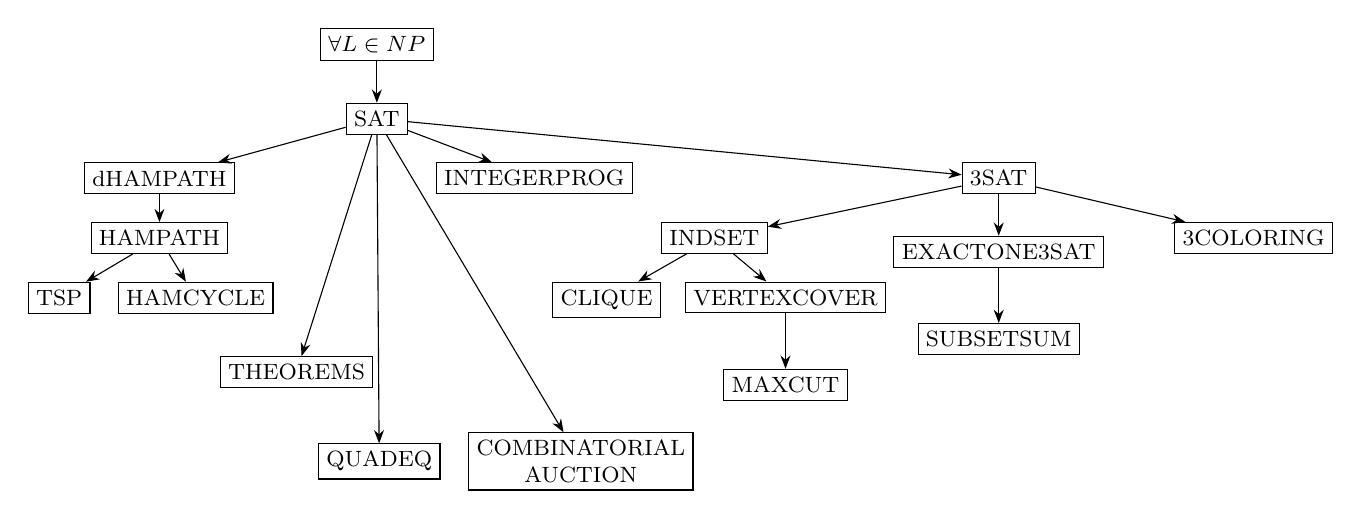
\begin{tikzpicture}[
    every node/.style={rectangle, draw, align=center}, 
    arrow/.style={-Stealth}
]
\centering
\footnotesize
\node (VLENP) {$\forall L \in NP$};
\node (SAT) [below=15pt of VLENP] {SAT};
\node (THREESAT) [below right=10pt and 200pt of SAT] {3SAT};
\node (THREECOL) [below right=10pt and 50pt of THREESAT] {3COLORING};
\node (EXACTONE3SAT) [below=15pt of THREESAT] {EXACTONE3SAT};
\node (SUBSETSUM) [below=20pt of EXACTONE3SAT] {SUBSETSUM};
\node (INDSET) [below left=10pt and 70pt of THREESAT] {INDSET};
\node (CLIQUE) [below left=10pt and 0pt of INDSET] {CLIQUE};
\node (VERTEXCOVER) [below right=10pt and -30pt of INDSET] {VERTEXCOVER};
\node (MAXCUT) [below=20pt of VERTEXCOVER] {MAXCUT};
\node (INTEGERPROG) [below right=10pt and 10pt of SAT] {INTEGERPROG}; 
\node (dHAMPATH) [below left=10pt and 40pt of SAT] {dHAMPATH};
\node (HAMPATH) [below=10pt of dHAMPATH] {HAMPATH};
\node (TSP) [below left=10pt and -0pt of HAMPATH] {TSP};
\node (HAMCYCLE) [below right=10pt and -40pt of HAMPATH] {HAMCYCLE};
\node (THEOREMS) [below left=80pt and -10pt of SAT] {THEOREMS};
\node (QUADEQ) [below right=20pt and -20pt of THEOREMS] {QUADEQ};
\node (COMBINATORIAL) [right=10pt of QUADEQ] {COMBINATORIAL\\AUCTION};
\draw [arrow] (VLENP) -- (SAT);
\draw [arrow] (SAT) -- (THREESAT);
\draw [arrow] (SAT) -- (INTEGERPROG);
\draw [arrow] (THREESAT) -- (EXACTONE3SAT);
\draw [arrow] (INDSET) -- (CLIQUE);
\draw [arrow] (EXACTONE3SAT) -- (SUBSETSUM);
\draw [arrow] (INDSET) -- (VERTEXCOVER);
\draw [arrow] (THREESAT) -- (INDSET);
\draw [arrow] (THREESAT) -- (THREECOL);
\draw [arrow] (VERTEXCOVER) -- (MAXCUT);
\draw [arrow] (SAT) -- (dHAMPATH);
\draw [arrow] (dHAMPATH) -- (HAMPATH);
\draw [arrow] (HAMPATH) -- (TSP);
\draw [arrow] (HAMPATH) -- (HAMCYCLE);
\draw [arrow] (SAT) -- (THEOREMS);
\draw [arrow] (SAT) -- (QUADEQ);
\draw [arrow] (SAT) -- (COMBINATORIAL);

\end{tikzpicture}
 (cite: Computational Complexity: A Modern Approach by Sanjeev Arora and Boaz Barak.)
    
    \newpage
    
    \titledquestion{Multiple Choice(s)}
For each multiple-choice, there may be \textbf{one or more} correct choice(s). Select all the correct answer(s). For each such question, you will get 0 points if you select \textbf{any} wrong choice, but you will get 1 point if you select a non-empty subset of the correct choices.
\textbf{Write your answers in the following table; otherwise, we may take your answers as unspecified.}\\
\textbf{Notice: ``must be true'' means the proposition holds no matter whether $\P = \NP$ or not. If you feel confused about some of the definitions, we encourage you to search the friendly web. But remember not to cheat or just use GenAI to fill in the blanks.}

%%%%%%%%%%%%%%%%%%%%%%%%%%%%%%%%%%%%%%%%%%%%%%%%%%%%%%%%%%%%%%%%%%%%%%%%%%%
% Note: The `LaTeX' way to answer a multiple-choices question is to replace `\choice' with `\choice', as what you did in the previous questions. 
% However, there are still many students who would like to handwrite their homework. To make TA's work 
% easier, you have to fill your selected choices in the table below, no matter whether you use LaTeX or not.
%%%%%%%%%%%%%%%%%%%%%%%%%%%%%%%%%%%%%%%%%%%%%%%%%%%%%%%%%%%%%%%%%%%%%%%%%%%

\begin{table}[htbp]
    \centering
    \begin{tabular}{|p{1.5cm}|p{1.5cm}|p{1.5cm}|p{1.5cm}|p{1.5cm}|p{1.5cm}|p{1.5cm}|}
        \hline
        2(a) & 2(b) & 2(c) & 2(d) & 2(e) & 2(f) & 2(g) \\
        \hline
        %%%%%%%%%%%%%%%%%%%%%%%%%%%%%%%%%%%%%%%%%%%%%%%%%%%%%%%%%%
        % YOUR ANSWER HERE.
          &   &   &   &   &   &  \\
        %%%%%%%%%%%%%%%%%%%%%%%%%%%%%%%%%%%%%%%%%%%%%%%%%%%%%%%%%%
        \hline
    \end{tabular}
\end{table}

\begin{parts}
\part[3] Choose those problems which must be in in $\complete{\NP}$:
\begin{choices}
    \choice $\mathsf{CYCLE}$: Given a graph $G=(V,E)$, check whether it has a cycle.
    \choice $\mathsf{GI}$: Given two graphs $G_1=(V_1,E_1)$ and $G_2 = (V_2,E_2)$, check whether $G_1$ is isomorphic to $G_2$. ($\exists f:V_1\to V_2$ is bijective and $(v_1,u_1)\in E_1$ if and only if $(f(v_1),f(u_1))\in E_2$). 
    \choice $\mathsf{K\text{-}COLORING}$: Given a graph $G=(V,E)$, check whether it has a $k$-coloring: $f:V\to [k]$ that $\forall e=(u,v)\in E, f(u)\not = f(v)$. ($k\geq 3$)
    \choice $\mathsf{KNAPSACK}$: Given $n$ items and a capacity $W$ where the weight and value of each item is $w_i$ and $v_i$ respectively. Check whether there is a subset of items such that the total weights of items are below $W$ and the total value are above $V$. ($n,w_i,W\in \mathbb{Z}^{+}, v_i, V\in \mathbb{R}^+$.)
\end{choices}

\part[3] Given two decision problems $A$ and $B$ such that there exists a polynomial-time many-one reduction from $A$ to $B$. Denote this as $A\leq_p B$. Which of the following statements must be true?
\begin{choices}
    \choice $A\in \P \implies B\in \P$
    \choice $A\in \complete{\NP} \implies B\in \complete{\NP}$.
    \choice $B\in \P\implies A\in \P$.
    \choice $B\in \complete{\NP} \implies A\in \complete{\NP}$.
\end{choices}

\part[3] Which of the following statements must be true? 
\begin{choices} 
    \choice Given a problem $A$, if there exists a polynomial-time certifier $f$ so that for any no-instance $X$ of $A$, there exists a polynomial-size certificate $u$, then $A$ is also in $\NP$.
    \choice If a problem $X$ can be solved in polynomial time in the range of the output result, then $X\in\P$.
    \choice If a problem $X$ can be solved in polynomial space in the length of the input result, then $X\in \P$.
    \choice $\P \neq \NP$ if and only if $\P \cap \complete{\NP} = \emptyset$.
    \choice $\P = \NP$ if and only if $\NP = \complete{\NP}$.
\end{choices}

\part[3] Which of the following statement(s) must be true? 
\begin{choices}
    \choice Every problem in $\NP$ can be solved in exponential time.
    \choice Finding a polynomial-time algorithm for problems in $\NP$ can prove $\P=\NP$.
    \choice There exists a polynomial-time many-one reduction from $\textsf{2\text{-}SAT}$ to every problem in $\NP$.
    \choice There exists a polynomial-time many-one reduction from every problem in $\NP$ to $\textsf{3\text{-}SAT}$.
\end{choices}

Given a problem set $L$, we call a problem $X$ in $\complete{L}$ if and only if every problem $Y\in L$ can be reduced to $X$ in polynomial time. Recall $\P$ and $\NP$ are defined on decision problems i.e. problems giving out $YES$ or $NO$. From this finish the following $2$ problems:

\part[3] Which of the following statement(s) of $\NP$ and $\complete{\NP}$ is/are true?
\begin{choices}
    \choice If $\exists L \in \complete{NP} \cap \P$, then $\P = \NP$.
    \choice If $L_1 \leq_p L_2, L_2 \leq_p L_3$, then $L_1\leq_p L_3$. Here $A\leq_p B$ means there exist a polynomial reduction from $A$ to $B$.
    \choice The $N$ in $\NP$ means ``No polynomial solutions" since $\P\not=\NP$ is mostly believed.
    \choice The $P$ in $\P$ means ``Polynomial'' since $X\in \P$ indicates $X$ can be solved in polynomial time.
\end{choices}

\part[3] Given a decision problem $A$ and its corresponding certifier C, the counting version of $A$, denoted as $\#A$, is defined such that for every instance x, the output of $\#A(x)$ is the number of certificates y for which $C(x,y)=1$. Specifically, $\#A(x)=|\{y|C(x,y)=1\}|$. Furthermore, $\#P$ is defined as $\#P=\{\#A|A\in\NP\}$. Which of the following statements must be true?
\begin{choices}
    \choice $\forall A\in \NP$, $A \in \complete{\NP}$ if and only if $\#A\in \complete{\#\P}$.
    \choice If $\# \SAT$ can be solved in polynomial time, then the decision problem $\P=\NP$. 
    \choice $\forall A\in \complete{\NP}$, $\#A\in\complete{\#\P}$.
    \choice If $\exists \#A\in \#\P$ can be solved in polynomial time, then $A\in \P$.
\end{choices}

\part[3] Which of the following statement(s) is/are true?
\begin{choices}
    \choice ``There exists an $\NP$ problem that is not an $\complete{\NP}$ problem.'' is false regardless of whether $\P$ equals to $\NP$ or not.
    \choice ``$\mathsf{Shortest\text{-}Path}$ is not in $\complete{\NP}$.'' is false regardless of whether $\P$ equals to $\NP$ or not.
    \choice ``There exists an $\NP$ problem that is not an $\complete{\NP}$ problem.'' is true if and only if $\P \neq \NP$.
    \choice ``$\mathsf{Shortest\text{-}Path}$ is not in $\complete{\NP}$.'' is true if and only if $\P \neq \NP$.
\end{choices}

\end{parts}

    
    \newpage
    
    \titledquestion{Dichotomy}

$\sat{3}$ is a well-known $\complete{\NP}$ problem and it has many variants. There exists a kind of dichotomy theorems due to the complexity problem defined by $S$ is either in $\P$ or is $\complete{\NP}$. Schaefer's dichotomy theorem shows that a large set of $\SAT$-like problems are $\complete{\NP}$, while only $6$ kinds of problems can be solved in polynomial time.

First of all we should claim some notations of $\SAT$(the Boolean satisfiability problem). Given a variable set $U = \{u_1,u_2,\cdots,u_n\}$, a \textbf{boolean formula} is defined as the combination of unary/binary operators $\vee$(OR), $\wedge$(AND), $\neg$(NOT) and the variables in the variable set $U$. Given a boolean formula $\phi$, if there exists a variable combination that makes $\phi$ true, then $\phi$ is satisfiable, otherwise $\phi$ is unsatisfiable.

A \textbf{SAT formula} is a logical formula in conjunctive normal form (CNF) Specifically, a \textbf{3-SAT formula} $\phi$ is a conjunction (AND) of clauses $C_1, C_2, \ldots, C_m$, and each clause $C_i$ is a disjunction (OR) of three literals (variables or their negations) from $X \cup \{\neg x_1, \neg x_2, \ldots, \neg x_n\}$. We will give out the initial $\complete{\NP}$ problem: $\sat{3}$.

$\sat{3}$: Given a set of Boolean variables $X = \{x_1, x_2, \ldots, x_n\}$ and a \textbf{3-SAT formula} $\phi$ on $X$, determine whether there exists at least one truth assignment $\tau$ that makes the formula $\phi$ evaluate to true. The yes-instance of $\sat{3}$ is:
\begin{equation*}
\mathsf{3\text{-}SAT} = 
\left\{\langle{\phi\rangle} \middle| 
\begin{aligned}
& \phi \text{ is a 3-SAT formula with variables } X = {x_1, x_2, \ldots, x_n}\\
&\text{and clauses } C_1, C_2, \ldots, C_m \text{ such that there exists} \text{ a truth } \\
& \text{assignment }\tau: X \rightarrow \{\text{true}, \text{false}\}\text{ such that } \tau(\phi) = \text{true}.
\end{aligned}
\right\}
\end{equation*}
In this problem, you are supposed to give out a reduction from the following problem to those problems in $\complete{\NP}$ if it is in $\complete{\NP}$, otherwise give out a polynomial time algorithm to solve it. Moreover, you are required to give out the yes-instances of those problems if they are in $\complete{\NP}$.
\begin{parts}
    \part[5] \textsf{Horn-SAT}: Given a set of Boolean variables $X = \{x_1, x_2, \ldots, x_n\}$ and a \textbf{Horn-formula} $\phi$ on $X$, determine whether there exists at least one truth assignment $\tau$ that makes the formula $\phi$ evaluate to true.

    A \textbf{Horn-fomula} is either a single literal (a positive or negative variable) or a disjunction of at most one positive literal and one or more negative literals. %In other words, Horn clauses are either unit clauses (single literals) or implications of the form $(A \rightarrow B_1 \land B_2 \land \ldots \land B_k)$, where $A$ is a positive literal and $B_1, B_2, \ldots, B_k$ are negative literals.

\begin{solution}

\end{solution}
\newpage
    \part[5]
    $\sat{4}$: Given a set of Boolean variables $X = \{x_1, x_2, \ldots, x_n\}$ and a \textbf{4-SAT formula}(a conjunction of clauses where each clause $C_i$ is a disjunction of $4$ literals) $\phi$ on $X$, determine whether there exists at least one truth assignment $\tau$ that makes the formula $\phi$ evaluate to true.
\begin{solution}
\\
\\
\\
\\
\\
\\
\\
\\
\\
\\
\\
\\
\\
\end{solution}
    \part[5]
    $\sat{(3,3)}$: Given a set of Boolean variables $X = \{x_1, x_2, \ldots, x_n\}$ and a \textbf{3-SAT formula} $\phi$ on $X$, where \textbf{each variable appears at most three times}, determine whether there exists at least one truth assignment $\tau$ that makes the formula $\phi$ evaluate to true.\\
    \textbf{Hint:} Consider how $a\Leftrightarrow b$ can be transformed into CNF. 
\begin{solution}
\\
\\
\\
\\
\\
\\
\\
\\
\\
\\
\\
\\
\\
 \end{solution}


\end{parts}
    
    \newpage

    \titledquestion{Carpenter's Rule}

In this problem, you need to prove is $\mathsf{Carpenter}$ in $\complete{\NP}$.

$\mathsf{Carpenter}$: Given an array \(L=[l_1,l_2,\cdots,l_n]\) of non-negative integers, determine whether there exists a sequence $D=[d_1,d_2,\cdots,d_n]$ where $d_i\in\{\pm 1\}$ such that $\max_{j=0}^n\{\sum_{i=1}^{j}d_il_i\}-\min_{j=0}^n\{\sum_{i=1}^{j}d_il_i\}\leq k$.

Intuitively speaking, give a sequence of rigid rods of various integral lengths connected end-to-end by hinges, can it be folded so that its overall length is at most $k$? Correspondingly, $l_i$ indicates the length of $i$-th rigid rod and $d_i$ indicates the direction of $i$-th rigid rod (fold left or right). The $\max$ and $\min$ indicate the leftmost and rightmost positions.

\begin{figure}[H]
    \centering
    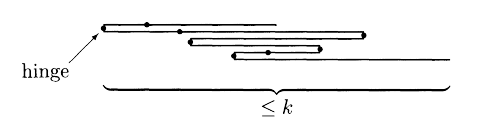
\includegraphics[width=0.5\linewidth]{hinge.png}
    \caption{Example of Hinge}
\end{figure}

The $yes$-instances of $\mathsf{Carpenter}$ is:
\begin{equation*}
\mathsf{Carpenter}= \left\{\langle{l_1, \ldots, l_{n},k\rangle}~\middle|~~~
\begin{aligned}
    & n\in \mathbb{Z}^+, l_1, \ldots, l_{n},k\in \mathbb{N},\exists D=[d_1,d_2,\cdots,d_n], d_i\in\{\pm 1\} \\ 
    & \text{i.e. }  D\in \{1,-1\}^{n} \text{ s.t. } \max_{j=0}^n\{\sum_{i=1}^{j}d_il_i\}-\min_{j=0}^n\{\sum_{i=1}^{j}d_il_i\}\leq k.
\end{aligned}
\right\}
\end{equation*}

\noindent We choose $\mathsf{Equivalent \text{-} Partition}$ to reduce from. Here is the $yes$-instance of it:
\begin{equation*}
\mathsf{Equivalent \text{-} Partition}= \left\{\langle{b_1, \ldots, b_{m}\rangle}~\middle|~~~\begin{aligned}
    &n\in \mathbb{Z}^+, b_1, \ldots, b_{m}\in \mathbb{N} \text{ and there exists a} \\ &\text{partition of the $b_i$'s to two parts whose sums}\\ &\text{are equivalent, i.e. }\exists{\:T\subseteq [m]}: \sum_{i\in T} b_i =  \sum_{j\in [m] \setminus T} b_j
\end{aligned}\right\}
\end{equation*}
Recall the definition of $\mathsf{Equivalent \text{-} Partition}$:

$\mathsf{Equivalent \text{-} Partition}$: Given an array \(B=[b_1,b_2,...,b_n]\) of non-negative integers, determine whether there exists a subset $T \subseteq [n]$ such that $\sum_{i\in T} b_i = \sum_{j \in [n] \setminus T} b_j $ (i.e. determine whether there is a way to partition $B$ into two disjoint subsets such that the sum of the elements in each subset is equivalent). 
\newpage
\begin{parts}
    \part[2] Prove that $\mathsf{Carpenter}$ is in $\NP$. (Show your certificate and certifier.)
    \begin{solution}\\
    Our certificate and certifier for $\mathsf{Carpenter}$ goes as follows:
    \begin{itemize}
        \item Certificate: 
        \item Certifier: 
    \end{itemize}
    \end{solution}

\part 
Consider how to construct your polynomial-time many-one reduction $f$ that maps instances of $\mathsf{Equivalent \text{-} Partition}$ to instances of $\mathsf{Carpenter}$. Unfortunately, the following reductions are not correct. Show that they are wrong by counterexamples.
\begin{subparts}
    \subpart[1] HaraoClesc gives out a reduction as follows: \\
    Let $n=m$ and $L=[l_1,l_2,\dots,l_n]$ be the sorted version in ascending order of $B=[b_1,\dots,b_m]$ i.e. $l_1$ is the minimum one in $B$, $a_n$ is the maximum of in $B$ and $l_i$ is the $i$-th minimum one in $B$ and $k = \frac12 \sum_{i=1}^{n}b_i$. Then $\aseq{l_1,\ldots,l_n,k}$ is a $yes$-instance of $\mathsf{Carpenter}$ if and only if $\aseq{b_1, b_2, \ldots, b_m}$ is a $yes$-instance of $\mathsf{Equivalent \text{-} Partition}$. 
    \begin{solution}\\\\
        \\
        \\
        \\
    \end{solution}
    \subpart[1] GeniusIdaiyo gives out another reduction as follows:
    Let $n=m+2$, then
        $$\aseq{l_1, \ldots, l_{n},k} = f(\aseq{b_1,\ldots,b_m}) \overset{\Delta}{=} \aseq{\max\{B\},b_1,\ldots,b_m,\max\{B\},\max\{B\}}$$ He deduces that $\aseq{l_1,\ldots,l_n,k}$ is a $yes$-instance of $\mathsf{Carpenter}$ if and only if $\aseq{b_1, b_2, \ldots, b_m}$ is a $yes$-instance of $\mathsf{Equivalent \text{-} Partition}$.
    \begin{solution}\\\\
\\
\\
\\
    \end{solution}
\end{subparts}
\newpage
\part From those wrong reductions above, FHKQ obtains a correct polynomial-time many-one reduction $f$ that maps instances of $\mathsf{Equivalent \text{-} Partition}$ to instances of $\mathsf{Carpenter}$. Show
\begin{subparts}
    \subpart[2] Your reduction in the format of (b).ii. (Show both $n$ and $L$.)\\
    \textbf{Hint:} Try to modify the above reductions into the correct one.
    \begin{solution}
\\
\\
\\
\\
\\
    \end{solution}
    \subpart[2]$x$ is a yes-instance of $\mathsf{Equivalent \text{-} Partition}\Rightarrow f(x)$ is a yes-instance of $\mathsf{Carpenter}$.
    \begin{solution}
\\
\\
\\
\\
\\
\\
\\
\\
\\
\\
\\
    \end{solution}
    \subpart[2]$f(x)$ is a yes-instance of $\mathsf{Carpenter}\Rightarrow x$ is a yes-instance of $\mathsf{Equivalent \text{-} Partition}$. 
    \begin{solution}
\\
\\
\\
\\
\\
\\
\\
\\
\\
\\
\\
    \end{solution}
\end{subparts}
\end{parts}





    \newpage

    \titledquestion{\textsc{Hamiltonian-Cycle} Problem}[9]
Show that the \textsc{Hamiltonian-Cycle} problem on the \textbf{undirected graph} is NP-complete. The \textsc{Hamiltonian-Cycle} problem is determining whether the graph $G$ contains a cycle that visits every vertex in $G$ exactly once. 

\textbf{Hint: } You can reduce this problem from the \textsc{D-Hamiltonian-Cycle} problem which determines whether there exists the Hamiltonian cycle on \textbf{the directed graph}.


\begin{solution}
\\\\\\\\\\\\\\\\\\\\\\\\\\\\\\\\\\\\\\\\\\\\\\\\\\\\\\\\
\end{solution}



\end{questions}

\end{document}
